\documentclass[12pt,a4paper]{article}

%\usepackage[left=1.5cm,right=1.5cm,top=1cm,bottom=2cm]{geometry}
\usepackage[in, plain]{fullpage}
\usepackage{array}
\usepackage{../../../pas-math}
\usepackage{../../../moncours}


%\usepackage{pas-cours}
%-------------------------------------------------------------------------------
%          -Packages nécessaires pour écrire en Français et en UTF8-
%-------------------------------------------------------------------------------
\usepackage[utf8]{inputenc}
\usepackage[frenchb]{babel}
\usepackage[T1]{fontenc}
\usepackage{lmodern}
\usepackage{textcomp}



%-------------------------------------------------------------------------------

%-------------------------------------------------------------------------------
%                          -Outils de mise en forme-
%-------------------------------------------------------------------------------
\usepackage{hyperref}
\hypersetup{pdfstartview=XYZ}
%\usepackage{enumerate}
\usepackage{graphicx}
\usepackage{multicol}
\usepackage{tabularx}
\usepackage{multirow}


\usepackage{anysize} %%pour pouvoir mettre les marges qu'on veut
%\marginsize{2.5cm}{2.5cm}{2.5cm}{2.5cm}

\usepackage{indentfirst} %%pour que les premier paragraphes soient aussi indentés
\usepackage{verbatim}
\usepackage{enumitem}
\usepackage[usenames,dvipsnames,svgnames,table]{xcolor}

\usepackage{variations}

%-------------------------------------------------------------------------------


%-------------------------------------------------------------------------------
%                  -Nécessaires pour écrire des mathématiques-
%-------------------------------------------------------------------------------
\usepackage{amsfonts}
\usepackage{amssymb}
\usepackage{amsmath}
\usepackage{amsthm}
\usepackage{tikz}
\usepackage{xlop}
%-------------------------------------------------------------------------------



%-------------------------------------------------------------------------------


%-------------------------------------------------------------------------------
%                    - Mise en forme avancée
%-------------------------------------------------------------------------------

\usepackage{ifthen}
\usepackage{ifmtarg}


\newcommand{\ifTrue}[2]{\ifthenelse{\equal{#1}{true}}{#2}{$\qquad \qquad$}}

%-------------------------------------------------------------------------------

%-------------------------------------------------------------------------------
%                     -Mise en forme d'exercices-
%-------------------------------------------------------------------------------
%\newtheoremstyle{exostyle}
%{\topsep}% espace avant
%{\topsep}% espace apres
%{}% Police utilisee par le style de thm
%{}% Indentation (vide = aucune, \parindent = indentation paragraphe)
%{\bfseries}% Police du titre de thm
%{.}% Signe de ponctuation apres le titre du thm
%{ }% Espace apres le titre du thm (\newline = linebreak)
%{\thmname{#1}\thmnumber{ #2}\thmnote{. \normalfont{\textit{#3}}}}% composants du titre du thm : \thmname = nom du thm, \thmnumber = numéro du thm, \thmnote = sous-titre du thm

%\theoremstyle{exostyle}
%\newtheorem{exercice}{Exercice}
%
%\newenvironment{questions}{
%\begin{enumerate}[\hspace{12pt}\bfseries\itshape a.]}{\end{enumerate}
%} %mettre un 1 à la place du a si on veut des numéros au lieu de lettres pour les questions 
%-------------------------------------------------------------------------------

%-------------------------------------------------------------------------------
%                    - Mise en forme de tableaux -
%-------------------------------------------------------------------------------

\renewcommand{\arraystretch}{1.7}

\setlength{\tabcolsep}{1.2cm}

%-------------------------------------------------------------------------------



%-------------------------------------------------------------------------------
%                    - Racourcis d'écriture -
%-------------------------------------------------------------------------------

% Angles orientés (couples de vecteurs)
\newcommand{\aopp}[2]{(\vec{#1}, \vec{#2})} %Les deuc vecteurs sont positifs
\newcommand{\aopn}[2]{(\vec{#1}, -\vec{#2})} %Le second vecteur est négatif
\newcommand{\aonp}[2]{(-\vec{#1}, \vec{#2})} %Le premier vecteur est négatif
\newcommand{\aonn}[2]{(-\vec{#1}, -\vec{#2})} %Les deux vecteurs sont négatifs

%Ensembles mathématiques
\newcommand{\naturels}{\mathbb{N}} %Nombres naturels
\newcommand{\relatifs}{\mathbb{Z}} %Nombres relatifs
\newcommand{\rationnels}{\mathbb{Q}} %Nombres rationnels
\newcommand{\reels}{\mathbb{R}} %Nombres réels
\newcommand{\complexes}{\mathbb{C}} %Nombres complexes


%Intégration des parenthèses aux cosinus
\newcommand{\cosP}[1]{\cos\left(#1\right)}
\newcommand{\sinP}[1]{\sin\left(#1\right)}


%Probas stats
\newcommand{\stat}{statistique}
\newcommand{\stats}{statistiques}
%-------------------------------------------------------------------------------

%-------------------------------------------------------------------------------
%                    - Mise en page -
%-------------------------------------------------------------------------------

\newcommand{\twoCol}[1]{\begin{multicols}{2}#1\end{multicols}}


\setenumerate[1]{font=\bfseries,label=\textit{\alph*})}
\setenumerate[2]{font=\bfseries,label=\arabic*)}


%-------------------------------------------------------------------------------
%                    - Elements cours -
%-------------------------------------------------------------------------------





%\makeatletter
%\renewcommand*{\@seccntformat}[1]{\csname the#1\endcsname\hspace{0.1cm}}
%\makeatother


%\author{Olivier FINOT}
\date{}
\title{Information chiffrée }

%\newcommand{\disp}{false}

\lhead{CH2 : Suites numériques}
\rhead{O. FINOT}
%
%\rfoot{Page \thepage}
\begin{document}
%\maketitle

\chap[num=2, color=red]{Suites numériques}{Olivier FINOT, \today }

\begin{myobj}
	\begin{itemize}
		
		\item Construire le symétrique d’un point ou d'une figure par rapport à une droite à la main où à l’aide d’un logiciel;
		\item Construire le symétrique d’un point ou d'une figure par rapport à un point, à la main où à l’aide d’un logiciel;
		\item Utiliser les propriétés de la symétrie axiale ou centrale;
		\item Identifier des symétries dans des figures.		
	\end{itemize}
\end{myobj}

\begin{mycomp}
	\begin{itemize}
		\item \kw{Chercher (Ch2)} :  s’engager    dans    une    démarche    scientifique, observer, questionner, manipuler, expérimenter (sur une feuille de papier, avec des objets, à l’aide de logiciels), émettre des hypothèses, chercher des exemples ou des contre-exemples, simplifier ou particulariser une situation, émettre une conjecture ;
		\item \kw{Raisonner (Ra3)} :  démontrer : utiliser un raisonnement logique et des règles établies (propriétés, théorèmes, formules) pour parvenir à une conclusion ;
		\item \kw{Communiquer (Co2)} :  expliquer à l’oral ou à l’écrit (sa démarche, son raisonnement, un calcul, un protocole   de   construction   géométrique, un algorithme), comprendre les explications d’un autre et argumenter dans l’échange ; 
		
	\end{itemize}
\end{mycomp}




\section{Suites numériques}

\begin{mydef}
	Une \kw{suite numérique} est constituée de \kw{plusieurs nombres rangés dans un certain ordre}. Ces nombres sont les \kw{termes} de la suite. $u_1$ est le premier terme de la suite, $u_2$ le deuxième, $u_n$ est le n-ième. Le terme suivant est noté $u_{n+1}$.\\
\end{mydef}

\section{Suites arithmétiques}

\subsection{Définition et terme de rang $n$}

\begin{myact}{La suite des nombres impairs}
	On considère la suite des nombres impairs, 1, 3, 5, 7, ..., que l'on note successivement $u_1$, $u_2$, $u_3$, $u_4$...
	Donc $u_1=1$, $u_2=3$, $u_3=5$...\\
	
	\begin{enumerate}[label=\arabic*)]
		\item \begin{enumerate}[label=\alph*.]
			\item Compléter : $u_4=.....$, $u_? =15$, $u_{10}=......$.
			\item Quel est le premier terme de la suite ?
			\item Comment passe-t-on d'un terme au suivant ?
			\item $n$ est est nombre entier positif non nul, on s'intéresse au terme de rang $n$ (donc le $n^{ième}$ nombre impair). Exprimer $u_{n+1}$ en fonction de $u_n$.
			\item Exprimer $u_n$ en fonction de $n$.
			\item Calculer $u_{100}$, $u_{150}$, $u_{1000}$.
		\end{enumerate} 
		
		\item Somme de nombres impairs. 
		
		On note $S_1=u_1=1$; $S_2=u_1+u_2=1+3=4$; puis, plus généralement $S_n=u_1+u_2+u_3+...+u_n$.
		
		\begin{enumerate}
			\item Compléter le tableau suivant :\\
			\begin{tabular}{|@{\ \ }l@{\ \ }|@{\ \ }c@{\ \ }|@{\ \ }c@{\ \ }|@{\ \ }c@{\ \ }|@{\ \ }c@{\ \ }|@{\ \ }c@{\ \ }|@{\ \ }c@{\ \ }|@{\ \ }c@{\ \ }|@{\ \ }c@{\ \ }|}
				\hline
				$n$   & 1 & 2 & 3 & 4 & 5 & 6 & 7 & 8 \\ \hline
				$u_n$ & 1 & 3 & 5 &   &   &   &   &   \\ \hline
				$S_n$ & 1 & 4 &   &   &   &   &   &   \\ \hline
			\end{tabular}
			
			\item En déduire une relation entre $S_{n+1}$, $S_{n}$, et $u_{n+1}$.
			
			\item En observant les résultats du tableau conjecturer une expression de $S_n$ en fonction de $n$.
		\end{enumerate}
	\end{enumerate}
	
	
\end{myact}

\begin{mybilan}
	\begin{itemize}
		
		\item Une \kw{suite arithmétique} est une suite de nombres, où chaque terme, à partir du deuxième est obtenu en ajoutant au précédent un même nombre, la \kw{raison} de la suite (notée $r$).	
		On note :
		\kw{{\LARGE \begin{align*}
					u_{n+1} = u_n + r 
				\end{align*}}}
			
			
			
		\item Dans une suite arithmétique de raison $r$, le terme $u_n$ est obtenu à partir du premier terme par la relation :
			\begin{itemize}
				\item \kw{$u_n = u_0 + nr$} (lorsque le terme initial est $u_0$) 
				\item \kw{$u_n = u_1 + (n-1)r$} (lorsque le terme initial est $u_1$)
			\end{itemize}
			

	\end{itemize}	
\end{mybilan}	

\subsection{Somme des termes d'une suite arithmétique}


\begin{myact}{Somme de nombres impairs}
	On note $S_1=u_1=1$; $S_2=u_1+u_2=1+3=4$; puis, plus généralement $S_n=u_1+u_2+u_3+...+u_n$.
	
	\begin{enumerate}
		\item Compléter le tableau suivant :\\
		\begin{tabular}{|@{\ \ }l@{\ \ }|@{\ \ }c@{\ \ }|@{\ \ }c@{\ \ }|@{\ \ }c@{\ \ }|@{\ \ }c@{\ \ }|@{\ \ }c@{\ \ }|@{\ \ }c@{\ \ }|@{\ \ }c@{\ \ }|@{\ \ }c@{\ \ }|}
			\hline
			$n$   & 1 & 2 & 3 & 4 & 5 & 6 & 7 & 8 \\ \hline
			$u_n$ & 1 & 3 & 5 &   &   &   &   &   \\ \hline
			$S_n$ & 1 & 4 &   &   &   &   &   &   \\ \hline
		\end{tabular}
		
		\item En déduire une relation entre $S_{n+1}$, $S_{n}$, et $u_{n+1}$.
		
		\item En observant les résultats du tableau conjecturer une expression de $S_n$ en fonction de $n$.
	\end{enumerate}
\end{myact}


		
		
	


\begin{mybilan}
	 $S_n$ est la somme des termes d'une suite arithmétique jusqu'à $u_n$, on a :
	\begin{itemize}
		\item \kw{$S_n = \dfrac{(n + 1) \times (u_0 + u_n)}{2} + nr$} (lorsque le terme initial est $u_0$) 
		\item \kw{$S_n = \dfrac{n \times (u_1 + u_n)}{2} + nr$} (lorsque le terme initial est $u_1$)
	\end{itemize}
\end{mybilan}


\newpage

\section{Suites Géométriques}

\subsection{Définition et terme de rang $n$}

\begin{myact}{Augmentation d'un loyer}
	Le loyer d'un appartement augmente chaque année de 3\%. En 2005, le loyer annuel s'élève à 6000 €.
	On note $v_n$, le montant du loyer annuel en $2005 + n$
	
	\begin{enumerate}
		\item Calculer le montant du loyer en 2006, 2007, 2008 et 2009.
		\item Quel est le premier terme de la suite ?
		\item Comment passe-t-on d'un terme au suivant ?
		\item Exprimer $v_{n+1}$ en fonction de $v_n$.
		\item Exprimer $v_n$ en fonction de $n$.
		\item Calculer $v_{10}$, $u_{15}$, $u_{35}$.
	\end{enumerate}
	
\end{myact}


\begin{mybilan}
	
	
	Une \kw{suite géométrique} est une suite de nombres, où chaque terme, à partir du deuxième est obtenu multipliant le précédent par un même nombre, la \kw{raison} de la suite (notée $q$).	
	
	On note :
	\kw{{\LARGE \begin{align*}
				u_{n+1} = u_n \times q 
	\end{align*}}}
	
	Dans une suite géométrique de raison $q$, le terme $u_n$ est obtenu à partir du premier terme par la relation :
	\begin{itemize}
		\item \kw{$u_n = u_0 \times q^n$} (lorsque le terme initial est $u_0$) 
		\item \kw{$u_n = u_1 \times q^{n-1}$} (lorsque le terme initial est $u_1$)
	\end{itemize}
	
%	\begin{multicols}{2}
%		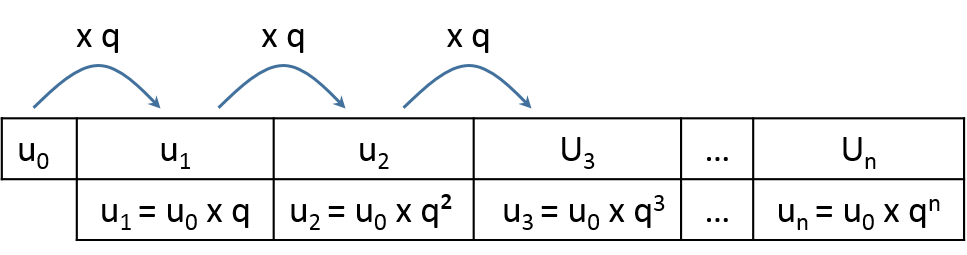
\includegraphics[scale=0.4]{./img/geo1}
%		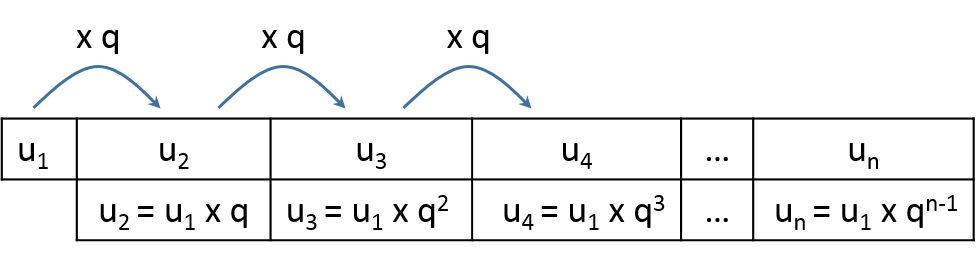
\includegraphics[scale=0.4]{./img/geo2}
%	\end{multicols}
%	
\end{mybilan}

\newpage 

\subsection{Sens de variation}

\begin{mybilan}
	Une suite géométrique de raison $q$ positive et de premier terme positif est :
	\begin{itemize}
		\item croissante, si $q > 1$;
		\item décroissante, si $q < 1$;
		\item constante, si $q = 1$.
	\end{itemize}
\end{mybilan}

\subsection{Somme de termes consécutifs d'une suite géométrique}

\begin{mybilan}
	 
	 $(u_n)$ est une suite géométrique de raison $q$, $S_n$ est la somme de ses termes jusqu'à $u_n$ ; on a :
	\begin{itemize}
		\item \kw{$S_n = u_0 \times \dfrac{1-q^{n + 1}}{1-q}$} (lorsque le terme initial est $u_0$) 
		\item \kw{$S_n = u_1 \times \dfrac{1-q^{n}}{1-q}$} (lorsque le terme initial est $u_1$)
	\end{itemize}
\end{mybilan}

\begin{myexs}
	\begin{enumerate}
		\item $(u_n)$ est la suite des puissances de 2 ($u_0 = 1$ et $q = 2$), on a :
		
		\begin{eqnarray*}
			S_8 &=& u_0 \times \frac{1 - q^{8+1}}{1 - q} \\
			S_8 &=& 1 \times \frac{1 - 2^9}{1 - 2} \\
			S_8 &=& 1 \times \frac{1 - 512}{1 - 2} \\
			S_8 &=& 511
		\end{eqnarray*} 
	
		\item $(v_n)$ est la suite définie par ($u_0 = \num{100000}$ et $q = \num{1.2}$), on a :
		
		\begin{eqnarray*}
			S_4 &=& u_0 \times \frac{1 - q^{4+1}}{1 - q} \\
			S_4 &=& \num{100000} \times \frac{1 - \num{1.2}^5}{1 - \num{1.2}} \\
			S_4 &=& \num{100000} \times \frac{1 - \num{2.48832}}{1 - \num{1.2}} \\
			S_4 &=& \num{744160}
		\end{eqnarray*} 
	\end{enumerate}
\end{myexs}
\end{document}